\chapter{Druck der Teile}
Im Folgenden wird der eigentliche 3D-Druck der Bauteile näher erläutert. Hierzu wird zunächst näher auf das Verfahren eingegangen, anschließend werden verschiedene Einstellungsmöglichkeiten bei der Erstellung der Steuercodes für den 3D-Drucker gezeigt.

\begin{figure}[h]
  \centering
  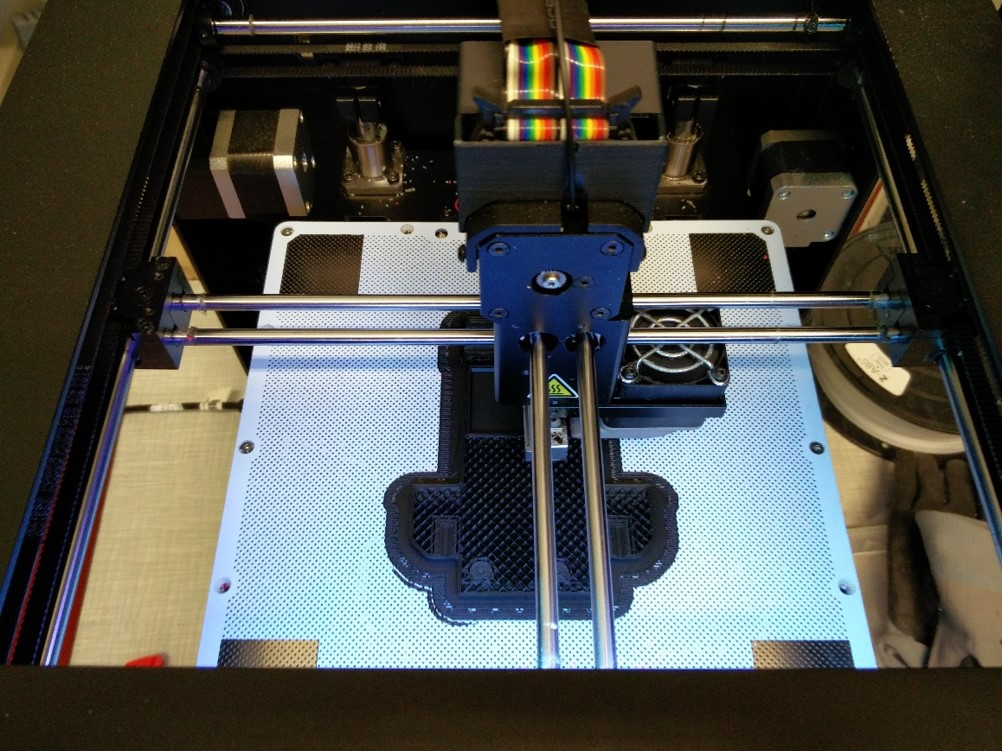
\includegraphics[width=12cm]{kapitel3/zortrax}
  \caption{Zortrax 3D-Drucker}
  \label{Kap3:Zortrax}
\end{figure}

\section{FDM}
Der Druck der Teile wurde bei dem hier vorgestellten Projekt nach dem \ac{FDM}-Verfahren durchgeführt, welches bereits 1989 durch S. Scott Crump mit der Firma Stratasys, Inc. patentiert\footnote{\cite{Crump1992}} wurde. Erst durch die auslaufenden Patentrechte wurde eine freie Verfügbarkeit ermöglicht. Auf diesem Verfahren basieren heute die Meisten 3D-Drucker in Preisklassen bis hin zum oberen Mittelfeld.

Bei dem \ac{FDM}-Verfahren wird das Ausgangsmaterial verflüssigt und durch eine ca. 0.4mm große Öffnung im Druckkopf gepresst. Durch eine Bewegung in 3-Achsen wird das flüssige Material in ca. 0.05 - 0.35mm dicken Schichten auf eine Plattform aufgetragen, dabei verschmelzen die Schichten miteinander und bilden das fertige Modell.

\begin{figure}[h]
  \centering
  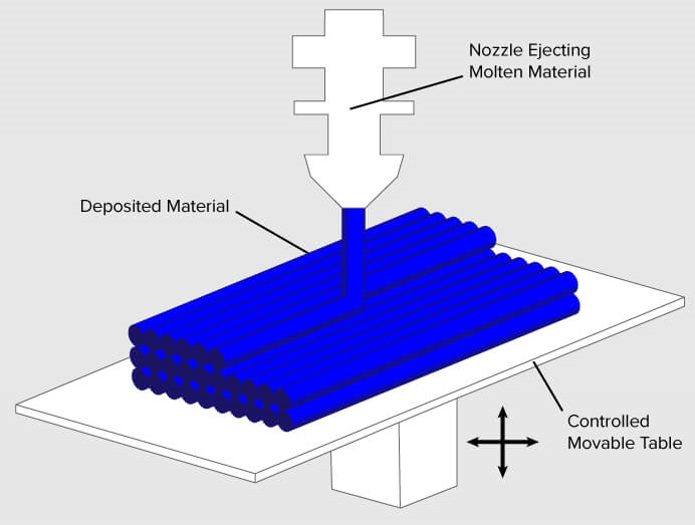
\includegraphics[width=14cm]{kapitel3/fdm}
  \caption{Visualisierung des FDM-Verfahrens}
  \source{\url{https://3dprinting.com/what-is-3d-printing/}}
  \label{Kap3:FDM}
\end{figure}

\section{Einstellmöglichkeiten}
Die Steuerbefehle (\textit{G-Code}) für den 3D-Drucker werden vom sog. \textit{Slicer} generiert. Dieser zerlegt das 3D-Modell in die einzelnen Schichten, generiert Stütz-, Füll- und Untergrundmaterial (\textit{Supports}, \textit{Infill} und \textit{Raft}) und definiert Parameter wie Temperatur, Geschwindigkeit und Extrusionsmenge.

\begin{figure}[h]
  \centering
  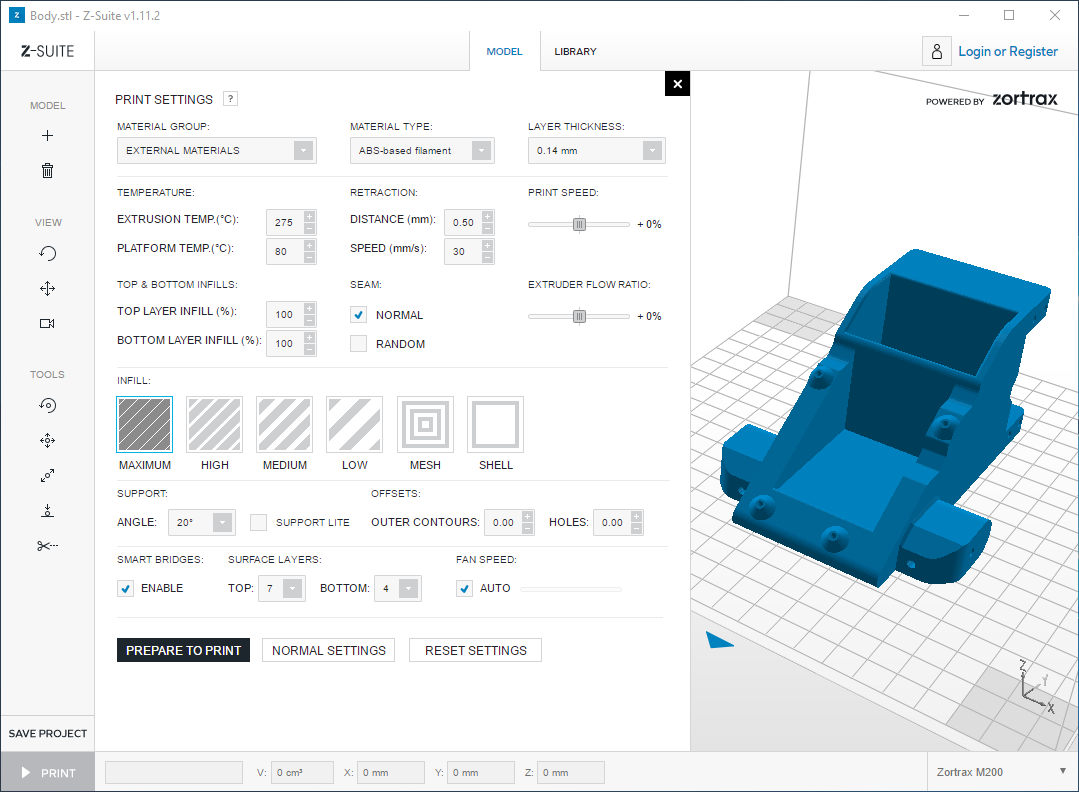
\includegraphics[width=9cm]{kapitel3/settings}
  \caption{Einstellmöglichkeiten}
  \source{Zortrax Z-Suite Slicer}
  \label{Kap3:Settings}
\end{figure}

\begin{figure}[h]
  \centering
  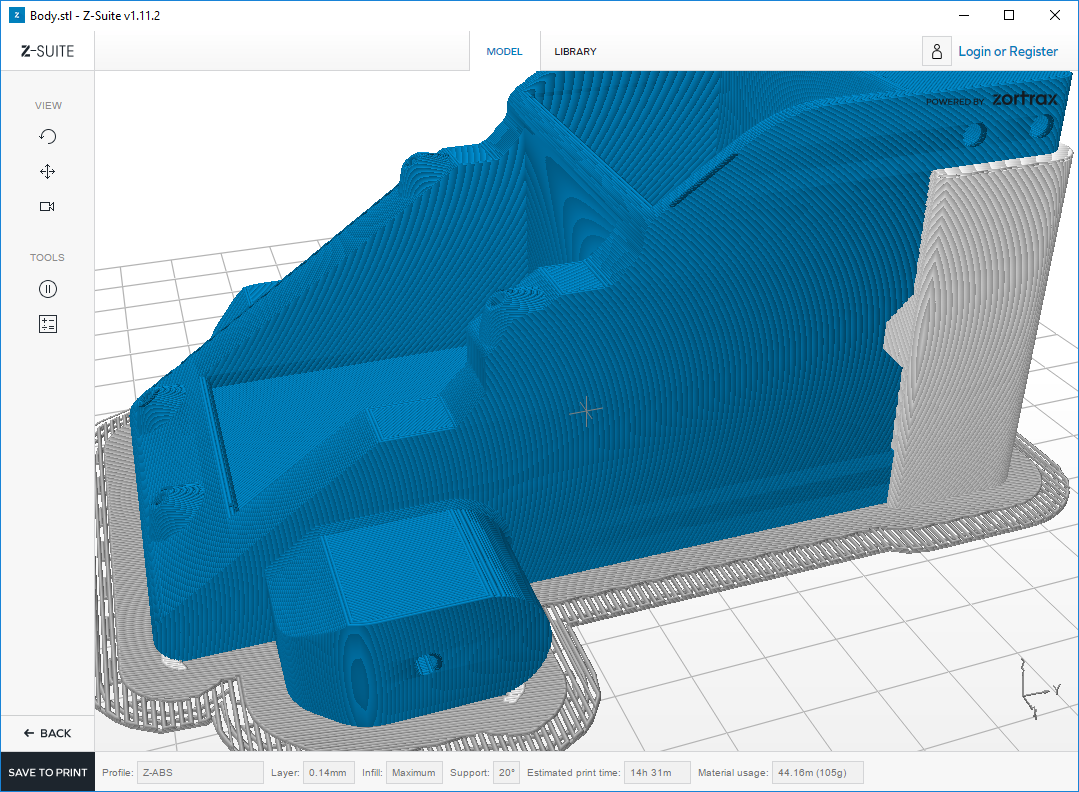
\includegraphics[width=9cm]{kapitel3/layers}
  \caption{Voransicht des G-Code -- \textbf{Unten:} Raft -- \textbf{Rechts:} Supports}
  \source{Zortrax Z-Suite Slicer}
  \label{Kap3:Preview}
\end{figure}

\section{Infill}
Gefüllte 3D-Modelle werden nur selten auch beim Druck mit Material gefüllt, stattdessen wird nur die äußere Hülle gedruckt und das Innere mit einem Muster gefüllt.

\begin{figure}[h]
  \centering
  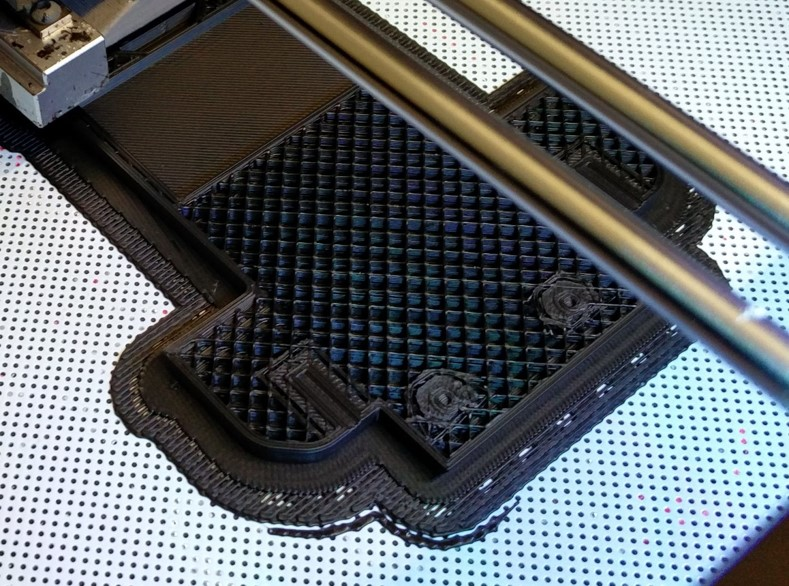
\includegraphics[width=12cm]{kapitel3/infill}
  \caption{Deutlich sichtbarer Infill während des Druckes}
  \label{Kap3:Infill}
\end{figure}

Dieses Muster ist der sog. \textit{Infill}. Er bietet einen Kompromiss aus Stabilität, Materialverbrauch, Druckdauer und Gewicht. Für diesen können die Dichte von 0 - 100 \% sowie ein Muster definiert werden. Dies dient vor allem der Verbesserung der Stabilität bei verschiedenen Arten der Belastung, Druckzeit und Materialverbrauch sind bei den meisten Mustern ähnlich.

\begin{figure}[h]
  \centering
  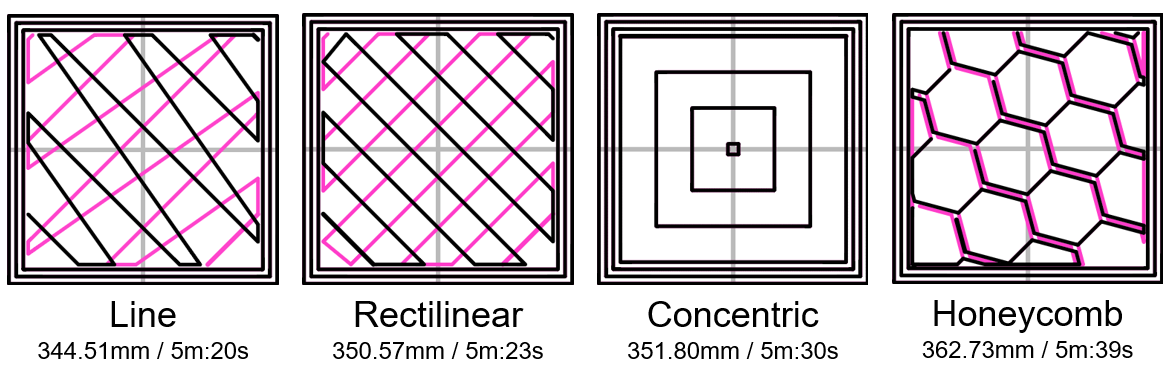
\includegraphics[width=14cm]{kapitel3/infilltype}
  \caption{Infill-Muster -- Materialverbrauch und Druckdauer für einen $20mm^3$ Würfel}
  \source{\url{http://manual.slic3r.org/expert-mode/infill}}
  \label{Kap3:Infilltype}
\end{figure}